\documentclass{frontiersSCNS}

%%%%% Some customizations

\usepackage{listings}
\usepackage{inconsolata}

\definecolor{dkgreen}{rgb}{0,0.6,0}
\definecolor{gray}{rgb}{0.5,0.5,0.5}
\definecolor{mauve}{rgb}{0.58,0,0.82}

\lstset{
  language=Python,
  aboveskip=3mm,
  belowskip=3mm,
  showstringspaces=false,
  columns=flexible,
  basicstyle={\small\ttfamily},
  numbers=none,
  numberstyle=\tiny\color{gray},
  keywordstyle=\color{blue},
  commentstyle=\color{dkgreen},
  stringstyle=\color{mauve},
  breaklines=true,
  breakatwhitespace=true,
  deletendkeywords={filter},
}

\graphicspath{{figures/}}

%%%%% Frontiers boilerplate

\usepackage{url,lineno}
% \linenumbers  % TODO uncomment!

\copyrightyear{2013}
\pubyear{2013}

\def\journal{Neuroinformatics}
\def\DOI{}
\def\articleType{Methods Article}
\def\keyFont{\fontsize{8}{11}\helveticabold }
\def\firstAuthorLast{Bekolay {et~al.}}
\def\Authors{Trevor Bekolay\,$^{1,*}$, James Bergstra\,$^{1}$,
  Eric Hunsberger\,$^{1}$, Travis DeWolf\,$^{1}$, Terrence C. Stewart\,$^{1}$,
  Daniel Rasmussen\,$^{1}$, Xuan Choo\,$^{1}$, Aaron Voelker\,$^{1}$,
  and Chris Eliasmith\,$^{1}$}
\def\Address{$^{1}$Computational Neuroscience Research Group,
  Center for Theoretical Neuroscience,
  University of Waterloo, Waterloo, ON, Canada}
\def\corrAuthor{Trevor Bekolay}
\def\corrAddress{David R. Cheriton School of Computer Science,
  University of Waterloo, 200 University Avenue West,
  Waterloo, ON, N2L 3G1, Canada}
\def\corrEmail{tbekolay@uwaterloo.ca}

%%%%% Document begins

\begin{document}
\onecolumn
\firstpage{1}

\title[Nengo in Python]{Nengo: A Python tool for
  building large-scale functional brain models}
\author[\firstAuthorLast ]{\Authors}
\address{}
\correspondance{}
\extraAuth{}
%\extraAuth{corresponding Author2 \\ Laboratory X2, Institute X2, Department X2,
%  Organization X2, Street X2, City X2 , State XX2
%  (only USA, Canada and Australia), Zip Code2, X2 Country X2, email2@uni2.edu}
\topic{Python in Neuroscience II}

\maketitle

\begin{abstract}
  Neuroscience currently lacks
  a comprehensive theory of
  how the brain implements cognitive processes
  with biological parts.
  The Neural Engineering Framework (NEF)
  proposes one such theory,
  but has not has not gathered
  significant empirical support
  due, in part, to the technical
  challenge of building and simulating
  large-scale models with the NEF.
  Nengo is a tool that builds and simulates
  functional brain models with the NEF.
  Nengo is the primary resource
  for teaching how the NEF
  is used to model neural systems,
  and for researchers using the NEF
  to build and simulate
  functional brain models.
  A previous version of Nengo was used
  to create Spaun,
  the world's largest functional brain model.
  The implementation of Spaun
  identified limitations
  in Nengo's ability to
  construct models with simple syntax,
  simulate them quickly,
  and collect data for subsequent analysis.
  We have implemented a new version of Nengo
  in Python that overcomes these limitations.
  It uses simple and extendable syntax,
  simulates a benchmark model on the scale of Spaun
  200 times faster than the previous implementation,
  and has a flexible mechanism
  for collecting simulation results.

  \tiny \keyFont{\section{Keywords:} Python, Neural Engineering
    Framework, theoretical neuroscience, computational neuroscience,
    control theory, software, simulation}
\end{abstract}

%max figures+tables: 15
%max legnth: 12000 words
%max pdf length: 12 pages

\section{Introduction}

It is often said that neuroscience
is data-rich but theory-poor.
Although computational neuroscience
has grown significantly,
this phrase continues to be repeated
due to a lack of satisfying
theories of the brain.
Much work has been put into neural simulators
that attempt to recreate neuroscientific
data in precise detail,
but behavior has not emerged
from data-driven large scale models.
Similarly, theoretical frameworks
consisting of a generic algorithm
replicated many times
(e.g., the memory-prediction framework \cite{TODO}
and the pattern recognition theory of mind \cite{TODO})
have not been shown to solve problems
that the generic algorithm alone cannot solve.

Nengo is a neural simulator
based on a theoretical framework proposed
by Eliasmith \& Anderson \citeyearpar{TODO}
called the Neural Engineering Framework
(NEF).
Nengo was recently used to implement Spaun,
currently the world's largest functional brain model
\cite{TODO}.
Spaun is a network of 2.5 million spiking neurons
that can perform eight high-level cognitive tasks
including list memory and inductive reasoning.
It can perform any of these eight tasks
at any time by being presented
the appropriate series of images
representing the task to be performed
and the details of that task;
for example, sequentially presenting images
containing the characters $A3[1234]$ instructs Spaun
to remember the list $1234$.
It then provides its answer by
sending motor commands to a simulated arm model,
tracing out digits.
If asked to recall the remember list,
it would trace out the digits $1234$.

While the tasks Spaun performs are diverse,
all tasks use a common set of
functional modules that we map
onto the brain areas hypothesized
to perform those functions.
Like data-driven large scale models,
Spaun is able to match experimental data
across the neuroscientific spectrum,
from the single cell to the behavioral level.
However, instead of constructing the model
based on data and hoping behavior emerges,
we construct the model
based on behavior
and see that the data emerges.
This is made possible by a theoretical framework
like the memory-prediction framework \cite{TODO},
but unlike it and other frameworks,
the NEF enables Spaun to employ
many different algorithms
based on the behavior being performed,
rather than defining a single algorithm
and hypothesizing that replicating it
many times will enable these behaviors.

In implementing Spaun,
we provided strong support
that the NEF is beginning to fill the theory void in neuroscience.
However, in doing so, we pushed Nengo
to the limits of its ability to construct and simulate
large-scale neural models.
In order to continue to evaluate the NEF
as a theory of the brain
by building larger and more complicated models,
we have begun the next generation
of Nengo with a focus on speed,
extensibility, and simplicity.

\subsection{JavaNengo limitations}

\begin{table}[!t]
\processtable{Tools bearing the name Nengo.\label{tab:nengo-vers}}
{\begin{tabular}{p{2.6cm} p{2.7cm} l p{7cm}} \toprule
\textbf{Name} & \textbf{Implementation language}
  & \textbf{Code repository} & \textbf{Purpose} \\\midrule
JavaNengo simulator & Java & \texttt{nengo\_java}
  & Simulates many types of spiking neuron models.
  Includes methods to construct and simulate models using the NEF. \\
JavaNengo GUI & Java & \texttt{nengo\_java\_gui}
  & Graphical interface to JavaNengo simulator.
  Allows modellers to drag-and-drop components built with the NEF. \\
JavaNengo scripting interface & Jython & \texttt{nengo\_jython}
  & Scripting interface to JavaNengo simulator.
  Provides shortcuts to classes and functions in the simulator.
  Also accessible through and interacts with the JavaNengo GUI. \\
PyNengo & Python & \texttt{nengo}
  & Constructs and simulates models using the NEF. \\
PyNengo OpenCL simulator & Python+PyOpenCL
  & \texttt{nengo\_ocl}
  & Simulates models constructed with PyNengo. \\\botrule
\end{tabular}}{Code repositories avilable at \url{http://github.com/ctn-waterloo/}.}
\end{table}

JavaNengo is a suite of tools providing
a neural simulator and graphical user interface (GUI)
implemented in Java,
and a scripting interface implemented in Jython
(see Table~\ref{tab:nengo-vers} for more detail).
JavaNengo's simulator was created
with the intention of being a general
neural simulator that included
the methods of the NEF
as one of several
methods for creating neural models.
As a result, its implementation
of important NEF components
are nested in deep class hierarchies,
adding unnecessary layers of complexity
for developers wishing
to extend those NEF components.
As a representative example,
the most often used class for making
NEF models, \texttt{NEFEnsemble},
extends from five ancestor classes
and implements seven interfaces.
Adding support for synaptic plasticity
in \texttt{NEFEnsemble}
involved adding or significantly modifying
25 Java classes \cite{TODO}.

The JavaNengo GUI provided
a drag-and-drop interface in which to create NEF models.
However, as it was developed
before the scripting interface,
the GUI manipulates simulator objects directly.
Typically, modellers start by following
tutorials that use the GUI interface,
and transition to the scripting interface
in order to implement more complicated models.
Since the GUI modifies simulator objects directly,
modelling concepts learned in the GUI
have to be relearned in the scripting interface.

The JavaNengo scripting interface,
described in \cite{TODO},
provided a simpler interface
to the NEF-specific portions of the simulator.
This greatly enhanced productivity,
and made it possible
to create many models with very little code.
Modellers quickly started using
the scripting interface
as their primary tool,
but still needed to access the GUI
for interactive model inspection,
and still needed to modify the simulator
to add new functionality
(e.g., to add new neuron models).
This is because Jython makes it easy
to inspect and create Java objects,
but does not make it easy to
write Java code to
inspect and create Jython objects.
Modellers, therefore, had to be
proficient in Java whether
they used the scripting interface or not.
As there are few neural modellers
that are proficient with both Java and Python syntax,
the scripting interface still lacks
convenient ways to record the results of simulations,
and to define complex experimental setups.
Additionally, Jython is always several versions
behind CPython, making it impossible
to use new language features
like dictionary comprehensions.
Jython also cannot access libraries
that contain any C code,
including all scientific libraries
that use NumPy.

Finally, perhaps the most significant limitation
of the JavaNengo tools is their performance.
While Java has good support for threads,
it does not have well-supported libraries
for doing mathematical operations on large matrices quickly.
Additionally, it is difficult to interface with
platform-specific tools such as
graphical processing units (GPUs),
which can perform the types of computations
that neural models require quickly and in parallel.

Addressing all of these issues
in the Java codebase would involve
significant enough changes
that we started from scratch instead.
Since the scripting interface
already used Python syntax,
and since Python is widely used
for neuroscientific data analysis,
we targeted the CPython interpreter
as the platform for the next generation of Nengo.

\subsection{PyNengo}

PyNengo,
the subject of the remainder of this paper,
is a Python package for
defining and simulating
neural models using the NEF.
It targets the CPython interpreter,
meaning that it integrates seamlessly
with other scientific Python tools.
Arbitrary CPython programs
can use Nengo models,
opening up possibilities
for using neurally implemented algorithms
in applications and games.

PyNengo's object model is simple and minimal,
making it easy to
document, test, and modify.
It also includes a scripting interface to those objects
based on JavaNengo's scripting interface \cite{TODO},
but with several modifications
to allow for easier incorporation
of user-defined networks,
new neuron models, and learning rules.
Additionally, PyNengo's scripting interface
contains methods to record simulated data
and access that data after simulation.

Model creation and simulation are decoupled,
allowing for models to be exported
to other simulators,
such as those accessible with PyNN.
Simulators can also be written
to leverage specific platforms.
Currently, we have implemented
a platform-independent simulator
that uses NumPy for vectorized computations,
and a PyOpenCL-based
simulator that takes full advantage of GPUs
and multicore CPUs.

PyNengo does not currently
replace all of JavaNengo's functionality.
While it can simulate the vast majority
of models that JavaNengo can simulate,
some functionality is still in development.
Most notably, there is no graphical interface
to PyNengo, and therefore simulations
cannot be visualized while they are running.
However, we are confident that these tools
can be created, and will be much easier
to implement compared to JavaNengo's GUI.

PyNengo overcomes all of JavaNengo's limitations.
It can simulate most models
currently simulated by JavaNengo
using 11\% as many lines of code,\footnote{
  JavaNengo is 40,000 lines of code, not including the GUI,
  and PyNengo is 5000 lines of code. TODO}
and depending on
only three external libraries instead of ten.
The OpenCL simulator can simulate
a large model TODO times
faster than JavaNengo's simulator.
This, along with a codebase
that is well tested and
easy to understand and extend,
provides a platform
that can simulate larger and more complex
models than Spaun,
and can therefore further
test the NEF as a theory of the brain.

\section{Neural Engineering Framework (NEF)}

The Neural Engineering Framework (NEF; \cite{TODO})
proposes three principles
that enable the construction
of large-scale neural models.

\begin{enumerate}
  \item \textbf{Representation:} A population of neurons
    collectively represents information in the form of
    time-varying vectors of real numbers.
  \item \textbf{Transformation:} Functions on those vectors
    are computed by the connections between populations.
  \item \textbf{Dynamics:} The vectors represented
    by neural populations can be considered state variables
    in a dynamical system, and can be analyzed using control theory.
\end{enumerate}

\begin{figure}
\begin{center}
  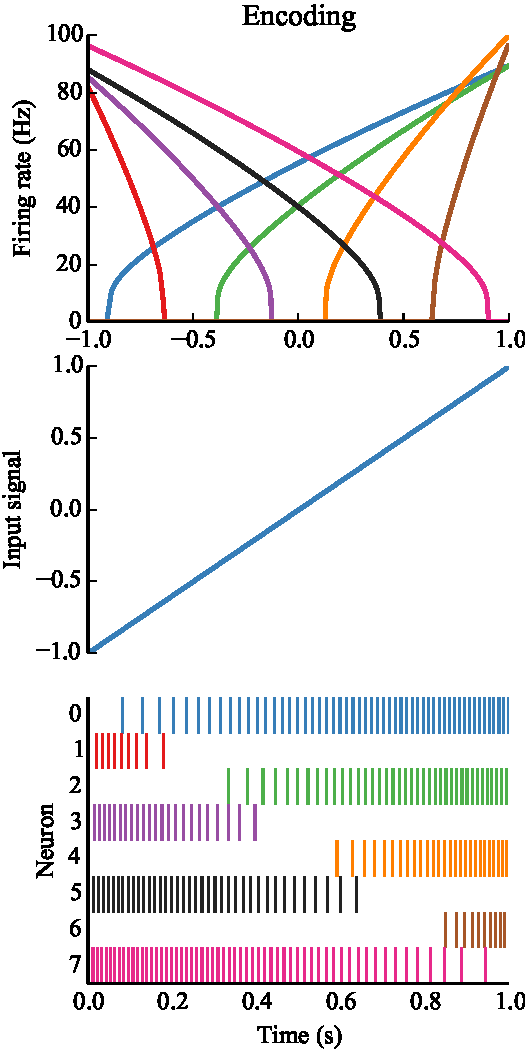
\includegraphics[width=0.245\textwidth]{nef_summary_enc}
  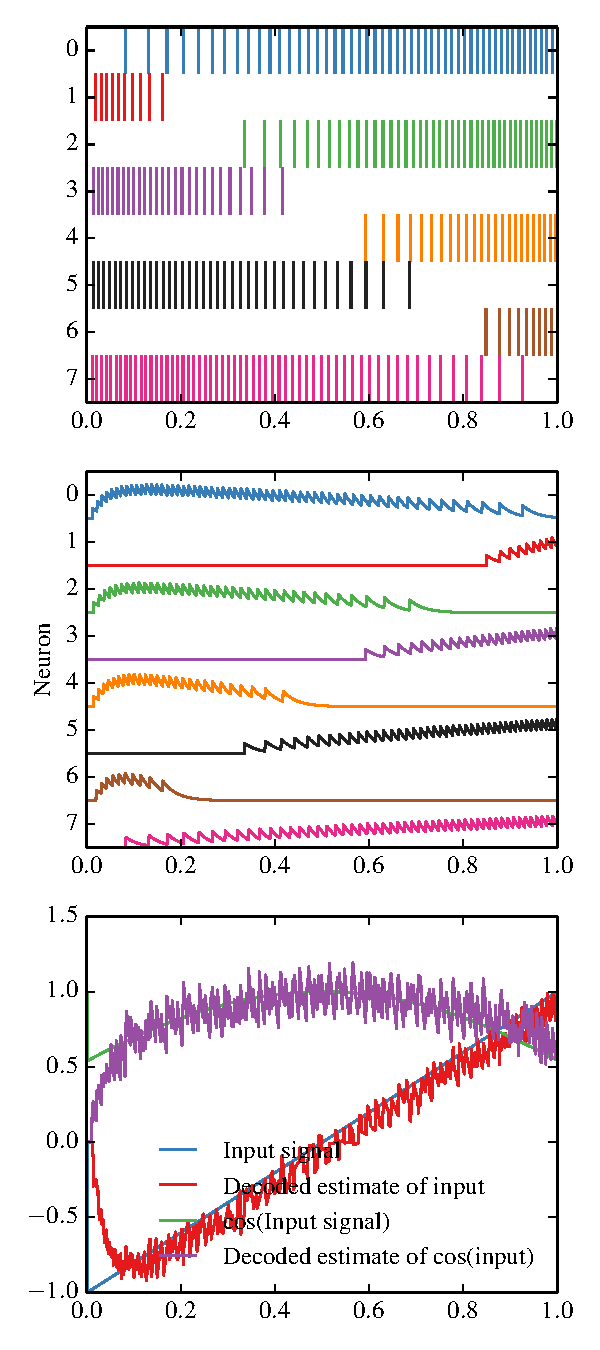
\includegraphics[width=0.245\textwidth]{nef_summary_dec}
  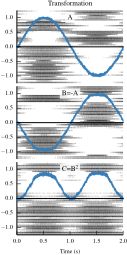
\includegraphics[width=0.245\textwidth]{nef_summary_trans}
  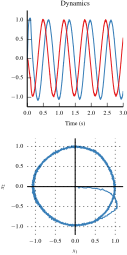
\includegraphics[width=0.245\textwidth]{nef_summary_dyn}
\end{center}
 \textbf{\refstepcounter{figure}\label{fig:nef} Figure \arabic{figure}.}{
   Summary of the three principles of the Neural Engineering Framework
   (NEF). (A) By the representation principle, signals are encoded
   in neural populations based on the \textit{tuning curve}
   of each neuron (top). The tuning curve describes
   how active a neuron is given some input signal.
   If we drive the eight neurons in the top panel
   with the input signal in the middle panel,
   we see the firing pattern in the bottom panel.
   (B) By the representation principle,
   the spiking activity of a neural population
   can be decoded to recover the original input signal,
   or some transformation of that input signal.
   First, the firing pattern shown in the top panel
   is filtered with a decaying exponential filter (middle panel).
   The filtered activity is then summed together
   with a set of weights that approximates
   the input signal (bottom panel, green)
   and the cosine of the input signal (bottom panel, purple).
   (C) By the transformation principle,
   populations of neurons can send signals
   to another population by decoding
   the desired function from the first population
   and then encoding the decoded estimate
   into the second population.
   These two steps can be expanded into a single step
   by calculating a set of weights
   that describe the strength of the connection
   between each neuron in the first population
   and each neuron in the second population.
   In (C), a sine wave is encoded by population A (top panel);
   the negative of that signal is projected
   to population B (middle panel)
   and the square of that signal is projected
   to population C (bottom panel).
   (D) By the dynamcs principle,
   signals being represented by population of neurons
   can be thought of
   as state variables in a dynamical system.
   In this example, the dynamical system
   has negative feedback across its two dimensions,
   resulting in a harmonic oscillator.
   The oscillator is plotted across time (top)
   and in state space (bottom).}
\end{figure}

\paragraph{Representation}
Information is encoded by populations of neurons.
We consider that information
to be time-varying vectors of real numbers,
in order to reason with that information
using conventional mathematics.
By doing this, we can \textit{encode}
those vectors by injecting
specific amounts of current into
single neuron models based on
the vector being encoded.
This drives the neuron,
causing it to spike.
We can then estimate
the originally encoded vector
through a \textit{decoding} process.
This idea is similar to population coding
\cite{TODO}, but generalized
to vectors of arbitrary length.

Figure~\ref{fig:nef} depicts
the encoding (A) and decoding (B) process.
In the encoding process, the input signal drives
each neuron based on its \textit{tuning curve},
which describes how much
that neuron fires for a given input signal.
The tuning curve summarizes the gain
of a neuron (how quickly the activity rises),
the bias (the activity of a neuron given no signal),
and the encoding weight
(the part of the vector space
that causes the neuron to fire most strongly).
This results in a predictable pattern of firing
given the input signal.

In the decoding process,
the spike trains are first filtered
with an exponentially decaying filter.
Those filtered spike trains are summed together
with weights that are determined
by solving a least-squares minimization problem.
In the bottom panel of Figure~\ref{fig:nef}B,
the red line is the filtered spiking activity
weighted by decoding weights
that minimize the difference between
the actual encoded vector
and the decoded estimate.
The purple line is the filtered spiking activity
weighted by decoding weights
that minimize the different between
the cosine of the actual encoded vector
and the decoded estimate.
Note that these decoding weights are not determined
based on the input signal;
instead, the minimization occurs
on points that are randomly sampled
in the vector space
that the population represents.

\paragraph{Transformation}
Neurons communicate through
unidirectional connections called synapses.
When a neuron spikes,
it releases neurotransmitter across the synapse,
which causes some amount of current
to be imparted in the downstream neuron.
Many factors affect the
amplitude of the current imparted;
we summarize those factors
in a scalar connection weight
representing the strength
of the connection between two neurons.
In order to compute any function,
we can set the connection weights between
two populations to be the product of
the decoding weights for that function
for neurons in the first population
and the encoding weights
for the downstream neuron.

In Figure~\ref{fig:nef}C,
a sine wave is transformed twice.
Between populations A and B,
the signal is negated.
Between populations B and C,
the signal is squared.

Note that, in practice, we rarely use
the full connection weight matrix,
and instead store
the encoding and decoding weights
(i.e., the factors of the connection weight matrix).
This provides significant
space and time savings.

\paragraph{Dynamics}
While doing feedforward transformations
on vectors is sufficient to model
many neural systems,
many systems, notably memory systems,
require persistent activity through recurrent connections.
When recurrent connection are introduced,
the vectors that populations represent
can be thought of as state variables
in a dynamical system.
Neural systems can therefore
be built and analyzed using
the methods of control theory.

In Figure~\ref{fig:nef}D,
a population represents a two-dimensional vector,
and is recurrently connected
with negative feedback between dimensions,
resulting in a harmonic oscillator.

\paragraph{Nengo}
Large models can be built
by thinking of the principles of the NEF
as building blocks that can be put together
to describe neural systems.
The goal of Nengo is to allow
modellers to describe neural systems
in terms of what information is being represented,
how that information is transformed,
and what dynamics are required
to perform cognitively relevant
functions with biologically constrained
neural components.
Those descriptions are then
translated to a network
of interconnected neurons.
This situates Nengo
as a ``neural compiler''
that translates
a high-level functional model
to a low-level neural model
that implements the high-level function.

\section{PyNengo object model}

\subsection{Model}

A Nengo model is a collection
of Nengo objects that represent information
and connections that transform information.
Objects and connections can be probed
in order to collect data during simulation.

The \texttt{Model} object is primarily a container
for Nengo objects,
but also doubles as a scripting interface
that simplifies creating, connecting,
and probing objects.
Basic models
can be created solely through interacting
with the \texttt{Model} object
(see sections \ref{sec:comm-channel}--\ref{sec:lorenz}
for examples).
In advanced models,
objects are instantiated
and then added to the model
(see section \ref{sec:cconv} for an example).

\subsection{Ensemble}

An \texttt{Ensemble} is
a population of neurons
that represents information
in the form of a real-valued vector.
An ensemble must be given as arguments
its dimensionality
(i.e., the length of the vector it represents),
and an object that describes
the population of neurons.
For example, \texttt{nengo.LIF(50, tau\_ref=0.002)}
describes a population
of 50 leaky integrate-and-fire neurons
with a refractory time of 0.002 seconds.
Neurons are defined symbolically
so that each simulator can compute
this population's nonlinear function
however it sees fit.
The neuron model used by the population
is easily changed, as long as the simulator
is aware of the neuron model description object.

Other attributes of the \texttt{Ensemble},
such as its encoding weights,
the maximum firing rate of its neurons,
and so on, can also be specified
either as keyword arguments
to the \texttt{Ensemble} constructor,
or by setting an attribute on the instantiated object.
While an ensemble makes a hypothesis
about the information being represented by neurons,
these additional attributes
also allow modellers to ensure that
the ensemble stays
within neurobiological constraints.
If these attributes are not set,
then they will be randomly selected
from distributions that describe
neocortical pyramidal cells.

\subsection{Node}

A \texttt{Node} tracks any information
that is not represented by an ensemble.
In the most common case,
nodes provide input signals
that drive ensembles of sensory neurons.
In a more general sense,
nodes represent the experimental environment
in which a neural model exists.

A node computes an arbitrary function
of its inputs directly.
Possible input signals include
the simulator timestep,
the decoded output of an ensemble,
or the output of another node.
However, unlike ensembles,
there are no constraints on the type
of function that the node computes.
A node can track any number of variables internally,
and use the state of those variables
when computing its function.
It can interact directly with hardware,
interface with other programs
using shared memory or sockets,
and so on.

Nodes allow many of the special-purpose
routines that are necessary in real-world
models to be integrated
as core components of a Nengo model.
This makes Nengo models more explicit,
and enables simulators
to control and optimize node execution.

\subsection{Connection}

Ensembles and nodes can be connected together
in several ways.
Like other objects in PyNengo's object model,
a connection contains symbolic information;
in this case, a connection tracks
how two objects are to be connected together.

The most important type of connection
in Nengo is the \texttt{DecodedConnection}.
This connection implements
the NEF's transformation principle.
In other words, the \texttt{DecodedConnection}
allows ensembles to project
the information they're representing---or
a transformation of that information---to
another ensemble or node.
This functionality is what enables Nengo models
to appear conceptual,
even though the underlying implementation
can translate that connection
to connection weights.

The ability to connect neurons together
with synaptic connection weights is still possible
with the \texttt{NonlinearityConnection}.
Both of these connection types
can be temporally filtered,
and the weights involved in the connection
(decoding weights for \texttt{DecodedConnection},
synaptic connection weights for \texttt{NonlinearityConnection})
can be modified over time with learning rules.

In many cases, the type of the connection
is not explicitly specified by the modeller.
Instead, it is inferred by the arguments
to \texttt{Model}'s \texttt{connect} function.
However, that function is just a simple wrapper
of each connection object's constructor,
so complex models can use
the appropriate connection,
or even implement their own.

\subsection{Network}

A network is a collection of ensembles and nodes
connected together in a particular way.
It is primarily a way of grouping together
a common set of connected objects,
and makes explicit the purpose
of the network and how it interacts
with the rest of the model
(see section \ref{sec:ccon} for a usage example).

Networks are designed to be
subclassed by users,
in order to group together
parts of a model.
In most cases,
the code that creates and connects
several objects in the model can be
moved into a \texttt{Network}
subclass' \texttt{make}
function with only minor changes.

Networks can vary dramatically in size,
and can be composed of other networks.
The \texttt{Integrator} network, for example,
is composed of only one recurrently connected ensemble.
By encapsulating that logic in a network,
the purpose of that ensemble is made explicit.
On the other end of the spectrum,
the \texttt{BasalGanglia} network
is composed of five groups of ensembles
connected with several specific functions
that together implement a ``winner-take-all'' circuit.
Encapsulating the code to create those ensembles
and connections in a network subclass
makes a complicated section of code
easy to include in many different models.

\subsection{Probe}

A probe marks that a signal
will be recorded
throughout the simulation.
Nengo objects and connections
each have several signals that can be probed.
An ensemble's decoded value
and its neurons' spikes
can be probed, among others.

Like nodes, a probe could be implemented
outside of the model.
However, doing so requires detailed knowledge
of the simulator,
and can incur significant overhead
if not implemented carefully.
For these reasons, we have made probes
a core component of a Nengo model,
and are therefore explicit
and optimizable.
Further, since probes are described
at a symbolic level,
the underlying implementation
can output probed data in many different formats.
Currently, simulators store probed data
directly in memory,
but adding the ability to store data
in files or to stream probed data
directly to sockets will be added.

\section{PyNengo simulators} \label{sec:simulators}

\begin{figure}
\begin{center}
  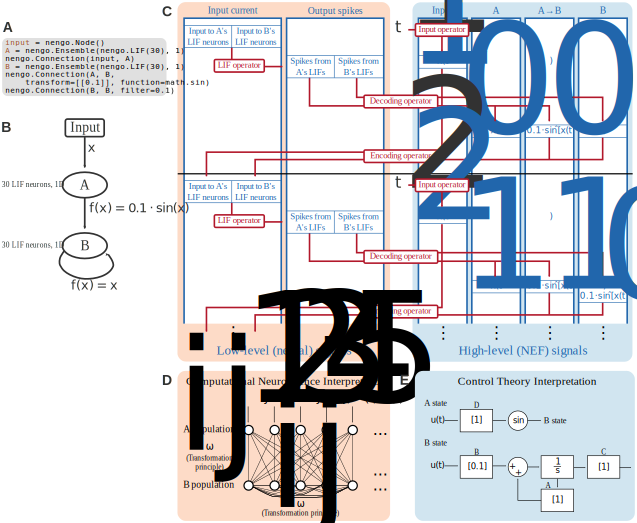
\includegraphics[width=\textwidth]{sim}
\end{center}
 \textbf{\refstepcounter{figure}\label{fig:sim} Figure \arabic{figure}.}{
   Detailed breakdown of the PyNengo reference simulator
   running a simple model for two timesteps.
   (A) Code describing the model being simulated.
   It consists of ensemble A project the sine of its
   encoded signal to ensemble B,
   which is recurrently connected.
   (B) Diagram depicting the model being simulated.
   (C) A detailed diagram of how the reference simulator
   simulates this model. Signals, which are the values
   tracked in the simulation, are colored blue.
   Operators, which are the computations done on signals,
   are colored red.
   Signals can be grouped as low-level neural signals
   that are used to compute the nonlinear functions
   underlying neuron models,
   and high-level NEF signals that are used to
   drive neurons and track the signals
   that the neurons are representing.
   The operators that implement the decoding
   and encoding steps map between
   the low-level neural signals
   and the high-level NEF signals.
   (D) The signals tracked at the low level
   can be interpreted as a model
   commonly seen in computational neuroscience literature;
   a population of leaky integrate-and-fire neurons
   is driven by some time-varying input current, $J(t)$.
   These neurons project to a population
   of recurrently connected neurons.
   The connection weight between the two populations,
   and from the second population to itself,
   can be computed by the NEF's transformation
   principle, bypassing the need for
   the high-level NEF signals
   used by the reference simulator
   for speed and data collection purposes.
   (E) The signals tracked at the high level
   can be interpreted as a dynamical system
   that can be analyzed with control theory.
   A simply represents its input,
   and passes its state to a sin function
   which becomes the input to B.
   B is a simple linear system
   that can be described with the typical
   $\dot{x}(t) = A x(t) + B u(t)$ equation.
   These dynamical systems can be simulated
   directly, without the use of spiking neurons,
   in order to quickly analyze system behavior.}
\end{figure}


Decoupling model creation and simulation
enables PyNengo simulators
to allocate memory and schedule computations
in the most efficient ways possible.
Simulators are given a \texttt{Model}
as an argument;
this \texttt{Model} is a symbolic description,
which a simulator can assume will not change
over the course of a simulation.
The simulator, however,
can modify the model as it sees fit;
in most cases, this means that the simulator
will fill in many of the details
that the symbolic description
has allowed to be generated randomly.

We have implemented
a reference simulator using NumPy
for vectorized computations,
and an OpenCL simulator
using PyOpenCL to parallelize
computations on GPUs and multicore CPUs.
In the remainder of this section,
we will describe
the reference simulator implementation;
the OpenCL simulator shares many
of the reference simulator's architectural choices,
but is heavily optimized in ways
that cannot be adequately described
with the space available.
Additionally, it should be noted that
any simulator that takes a \texttt{Model}
as input and exposes a \texttt{step}
function can be used in PyNengo;
the reference simulator
is provided as an example
for simulator designers,
not as a specification.

Before the first timestep, the reference simulator
\begin{enumerate}
  \item translates high-level objects to
    a set of signals and operators,
  \item allocates NumPy arrays for each signal, and
  \item sorts operators based on a dependency graph.
\end{enumerate}
On each timestep, the reference simulator
\begin{enumerate}
  \item computes each operator in order, and
  \item copies probed signals to a separate buffer.
\end{enumerate}
Figure~\ref{fig:sim} depicts
the state of the reference simulator
after two timesteps of a simple model.

\paragraph{Signals}

A \texttt{Signal} represents any number that
will be used by the simulator.
Each high level Nengo object contains
several signals;
for example, an ensemble contains signals
that represent the high-level input
signal that will be encoded
to input currents,
and the encoding weights.
It also contains a neural population,
which contains signals that represent
input currents, bias currents,
membrane voltages, and refractory times for each cell.

As can be seen in Figure~\ref{fig:sim},
the signals used in a Nengo simulation
can be conceptually grouped into
those that track low-level neural signals,
and those that track high-level signals
defined by the NEF.
Most neural simulators only track
low-level signals.
Operators commonly map
between related low- and high-level signals.

\paragraph{Operators}

Operators represent computations
to be performed on signals on each timestep.
Once the model has been built,
only a small set of mathematical
operations are necessary for simulation.

Many of the computations
done in a simulation
are linear (e.g.,
the decoding and encoding steps
in Figure~\ref{fig:sim}),
and therefore can share a common operator;
this can be helpful for parallelization
in some simulators.

Nonlinear functions, however,
require specific operators.
Each supported neuron model and learning rule
has an associated operator;
the simulator explicitly maps
from symbolic neuron objects in ensembles
and from symbolic learning rule objects
in connections to their associated operator.

\section{Examples} \label{sec:examples}

\subsection{Communication channel} \label{sec:comm-channel}

\begin{figure}
\begin{center}
  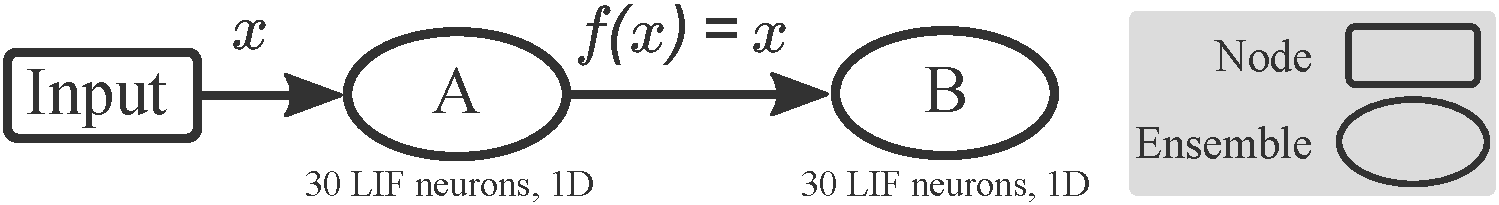
\includegraphics[width=.85\textwidth]{comm_channel}
  \begin{minipage}{0.48\textwidth}
    \begin{lstlisting}
import nengo
from nengo.helpers import white_noise
model = nengo.Model("Communication Channel")
model.make_node("Input", white_noise(1, 5))
model.make_ensemble("A", nengo.LIF(30), 1)
model.make_ensemble("B", nengo.LIF(30), 1)
model.connect("Input", "A")
model.connect("A", "B")
model.probe("Input")
model.probe("A", filter=0.01)
model.probe("A.spikes")
model.probe("B", filter=0.01)
model.probe("B.spikes")
sim = model.simulator()
sim.run(1)
A_data = sim.data("A")
A_spikes = sim.data("A.spikes")
...
    \end{lstlisting}
  \end{minipage}
  \begin{minipage}{0.39\textwidth}
    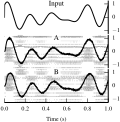
\includegraphics[width=\textwidth]{comm_channel_res}
  \end{minipage}
\end{center}
 \textbf{\refstepcounter{figure}\label{fig:comm-channel}
   Figure \arabic{figure}.}{
   A communication channel implemented with Nengo.
   (A) Diagram depicting the model. Ensemble A
   projects its encoded signal to ensemble B unchanged.
   (B) Nengo code to build and simulate the model
   for 1 second.
   (C) The results of the simulation.
   The input signal (top panel) is white noise limited to 0 to 5 Hz.
   The signal is well represented by both ensemble A (middle panel)
   and ensemble B (bottom panel) despite the neural firing patterns
   (underlaid in middle and bottom panels) being different.}
\end{figure}

A communication channel
is a minimal example demonstrating
the representation and transformation principles
of the NEF.
A communication channel
represents some signal and transmits it unchanged;
i.e., it computes the function $f(x) = x$.
Figure~\ref{fig:comm-channel}
depicts a scalar communication channel
representing band-limited Gaussian white noise.

The communication channel
is a simple enough model
that it can be readily implemented in PyNN.
Figure~\ref{fig:pynn} contains the code
for implementing a communication channel in PyNN.
This highlights many of the differences
between Nengo models and conventional neural models;
we also use the script for benchmarking
(see section \ref{sec:benchmark}).

\begin{figure}
\begin{center}
  \begin{minipage}{.435\textwidth}
    \begin{lstlisting}[basicstyle={\footnotesize\ttfamily}]
# We use Nengo to generate
#     bias: Bias currents
#     decoders: Decoding weights
#     encoders: Encoding weights
# for populations A and B.
import pynn.nest as pyNN

lif_params = {'tau_refrac': 2.0, 'tau_syn_E':100,
               'tau_syn_I':100}
dt = 0.5
pyNN.setup(timestep=dt, min_delay=dt)
A = pyNN.Population(30, pyNN.IF_cond_exp, lif_params)
B = pyNN.Population(30, pyNN.IF_cond_exp, lif_params)
input_signal = 0.5
inputA = [pyNN.DCSource(amplitude=val) for val
           in A_bias + input_signal * A_encoders]
for i, pulse in enumerate(inputA):
    pulse.inject_into(A[i:i+1])
inputB = [pyNN.DCSource(amplitude=val) for val
           in B_bias]
for i, pulse in enumerate(inputB):
    pulse.inject_into(B[i:i+1])
    \end{lstlisting}
  \end{minipage}
  \begin{minipage}{.46\textwidth}
    \begin{lstlisting}[basicstyle={\footnotesize\ttfamily}]
weights = []
for i in xrange(30):
    for j in xrange(30):
        weights.append((i, j,
            np.dot(A_decoder[i], B_encoder[j]), 1.0))
connection = pyNN.Projection(
    A, B, pyNN.FromListConnector(weights))
A.record('spikes')
B.record('spikes')
pyNN.run(1000)

# Decoded value of B
B_output = numpy.zeros(1000)
for i in xrange(1000):
    spikes = B[i:i+1].getSpikes()[:,1]
    spikes = (spikes / dt).astype('int')
    B_output[spikes] += B_decoder[i]
# Filter with tau = 200 ms
decay = np.exp(-dt / 200)
B_output[0, :] *= (1 - decay)
for i in xrange(1, 1000):
    B_output[i,:] = decay * B_output[i-1,:]
                     + (1-decay) * B_output[i,:]
    \end{lstlisting}
  \end{minipage}
\end{center}
 \textbf{\refstepcounter{figure}\label{fig:pynn} Figure \arabic{figure}.}{
   Implementation of the communication channel in PyNN.
   Note that several quantities are generated from Nengo;
   the functions that generate these quantities in Nengo
   can be decoupled, but are not included here for brevity.
   The implementation of the Lorenz attractor
   is not shown, but is very similar to the communication channel.}
\end{figure}

\subsection{Lorenz attractor network} \label{sec:lorenz}

\begin{figure}
\begin{center}
  \begin{minipage}{0.43\textwidth}
    \begin{lstlisting}[basicstyle={\footnotesize\ttfamily}]
import nengo
tau = 0.1; sigma = 10; beta = 8.0/3; rho = 28
model = nengo.Model('Lorenz attractor')
model.make_ensemble('State', nengo.LIF(2000),
                      dimensions=3, radius=60)

def feedback(x):
    dx0 = -sigma * x[0] + sigma * x[1]
    dx1 = -x[0] * x[2] - x[1]
    dx2 = x[0] * x[1] - beta * (x[2] + rho) - rho

    return [dx0 * tau + x[0],
            dx1 * tau + x[1],
            dx2 * tau + x[2]]

model.connect('State', 'State',
                function=feedback, filter=tau)
model.probe('State', filter=tau)
model.probe('State.spikes')
sim = model.simulator()
sim.run(6)
    \end{lstlisting}
  \end{minipage}
  \begin{minipage}{0.55\textwidth}
    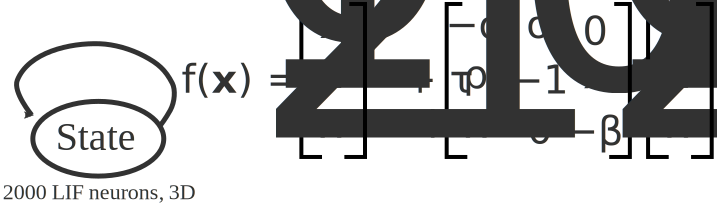
\includegraphics[width=0.95\textwidth]{lorenz}
    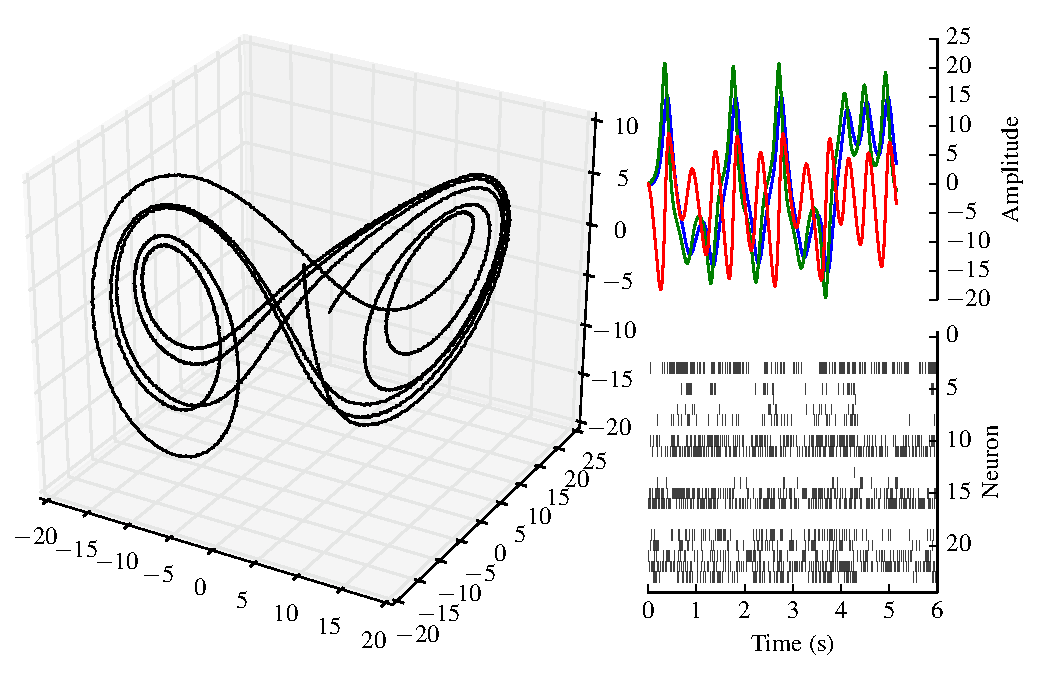
\includegraphics[width=\textwidth]{lorenz_res}
  \end{minipage}
\end{center}
 \textbf{\refstepcounter{figure}\label{fig:lorenz} Figure \arabic{figure}.}{
   A Lorenz attractor implemented with Nengo.
   (A) Nengo code to build and simulate the model
   for 6 seconds.
   (B) Diagram depicting the model. The state ensemble
   is recurrently connected with complex dynamics
   implemented the chaotic Lorenz attractor.
   Not that this populations does not receive
   any input that might drive its initial value;
   instead, the initial value is determined by
   the baseline firing of the 2000 leaky integrate-and-fire
   neurons that make up the state ensemble.
   (C) The trajectory that the state ensemble takes
   in its three-dimensional state space.
   For the parameters chosen, the trajectory takes
   the well-known butterfly shape.
   (D) The state vector plotted over time.
   (E) The spikes emitted by a random sample of 25
   neurons from the state ensemble.
   Some neurons fire uniformly across the 6 second simulation,
   but most change depending on the state being tracked
   due to the recurrent connection.}
\end{figure}

Many models in theoretical neuroscience
are based on attractor networks.
The NEF has been used in the past
to implement many different types of
attractor networks \cite{TODO}.
Figure~\ref{fig:lorez} depicts
a Nengo implementation of the Lorenz chaotic attractor
with a single ensemble
composed of 2000 leaky integrate-and-fire neurons.

We have implemented the Lorenz attractor
in PyNN for benchmarking purposes
(see supplementary material).

\subsection{Circular convolution} \label{sec:cconv}

\begin{figure}
\begin{center}
  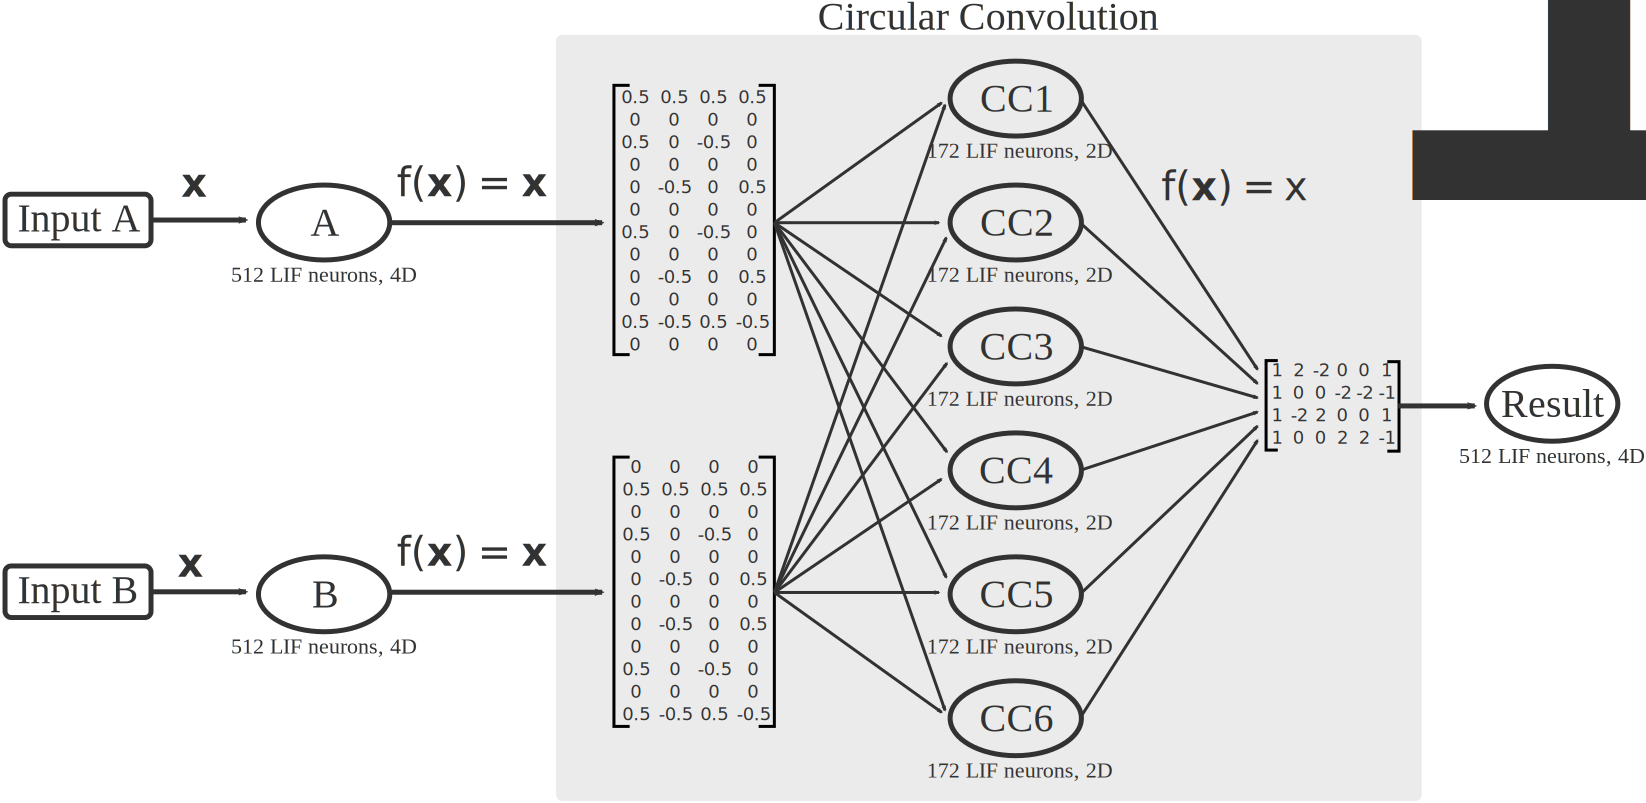
\includegraphics[width=0.8\textwidth]{cconv}
  \begin{minipage}{0.46\textwidth}
    \begin{lstlisting}[basicstyle={\footnotesize\ttfamily}]
import nengo
from nengo.networks import CircularConvolution
model = nengo.Model("Circular convolution")
model.make_node("Input A", [-0.21, 0.5, 0.12, 0.06])
model.make_ensemble("A", nengo.LIF(512), 4)
model.connect("Input A", "A")
model.make_node("Input B", [-0.18, 0.28, 0.18, -0.52])
model.make_ensemble("B", nengo.LIF(512), 4)
model.connect("Input B", "B")
cconv = model.add(CircularConvolution("Circular Convolution",
    neurons=nengo.LIF(1032), dimensions=4))
model.connect("A", cconv.A)
model.connect("B", cconv.B)
model.make_ensemble("Result", nengo.LIF(512), 4)
model.connect(cconv, "Result")
model.probe("A", filter=0.02)
model.probe("B", filter=0.02)
model.probe("Result", filter=0.02)
sim = model.simulator()
sim.run(0.5)
    \end{lstlisting}
  \end{minipage}
  \begin{minipage}{0.46\textwidth}
    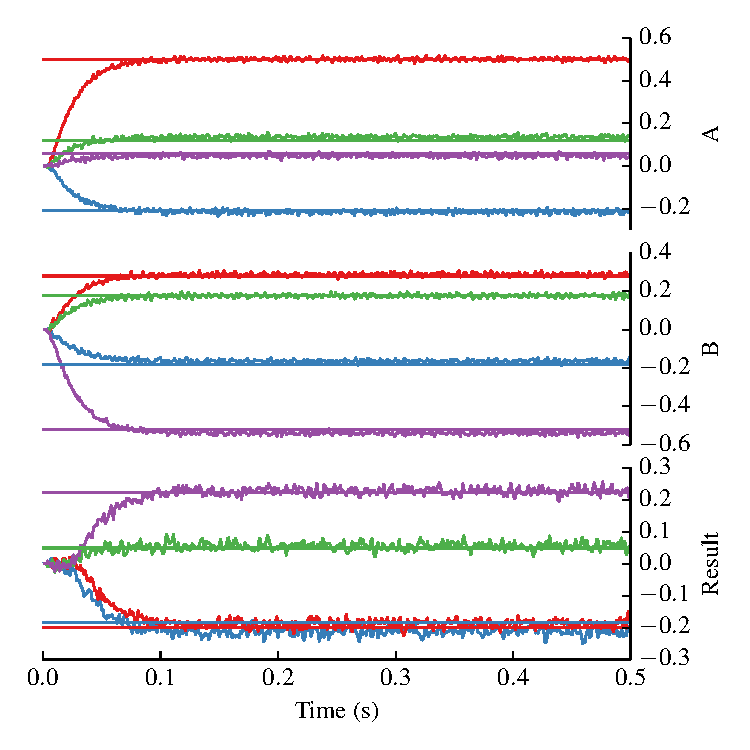
\includegraphics[width=\textwidth]{cconv_res}
  \end{minipage}
\end{center}
 \textbf{\refstepcounter{figure}\label{fig:cconv} Figure
   \arabic{figure}.}{
   Circular convolution implemented with Nengo.
   (A) Diagram depicting the model.
   The input vectors, A and B, represent four-dimensional signal
   which are mapped onto six ensembles within the
   Circular Convolution network through
   a complicated transformation matrix.
   Each ensemble within the network represents a
   two-dimensional signal. The product of those two signals
   is projected through another complicated transformation matrix
   to compute the final four-dimensional result.
   Note that the complicated parts of the model
   are contained within the network;
   the number of ensembles and the transform matrices shown
   are automatically generated by the network depending on
   the dimensionality of the input vectors.
   (B) Nengo code to build and simulate the model
   for 0.5 seconds.
   (C) The result of the simulation.
   Straight horizontal lines represent
   the target values that each ensemble
   should represent.
   Wavy lines represent the decoded values
   for each dimension represented by the
   A, B, and Result ensembles
   (top, middle, bottom panels respectively).
   The ensembles represent the correct values,
   after a startup transient of less than 0.1 seconds.}
\end{figure}

One of the most common operations done
in Nengo models is circular convolution.
Circular convolution is how
the semantic pointer architecture
(SPA; \cite{TODO})
binds two semantic pointers together.
Binding is central to many
of the high level cognitive tasks
that make Spaun unique.
Circular convolution
is best implemented in a two-layer network,
rather than in a single connection.
This two-layer network construction is simplified
by the existence of the \texttt{CircularConvolution} network.
The complexity encapsulated in that network
can be seen in Figure~\ref{fig:cconv}.

Unlike the previous two examples,
we do not implement
circular convolution in PyNN.
The resulting script would be
too long to be instructive.

\section{Benchmarks}

\begin{figure}
\begin{center}
  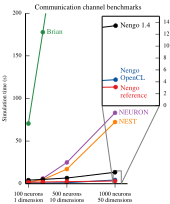
\includegraphics[width=0.32\textwidth]{bench_cchannel}
  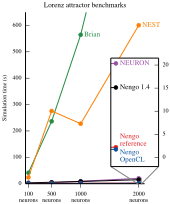
\includegraphics[width=0.32\textwidth]{bench_lorenz}
  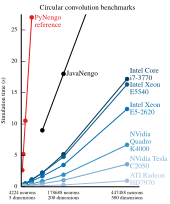
\includegraphics[width=0.32\textwidth]{bench_cconv}
\end{center}
 \textbf{
     \refstepcounter{figure}\label{fig:benchmarks}
     Figure \arabic{figure}.}{
     For (A) and (B), all of the simulators
     except the PyNengo OpenCL simulator
     was run on an Intel Core i7-965.
     JavaNengo used all 4 cores of this processor;
     all other simulator used only 1 core.
     The PyNengo OpenCL simulator
     was run on an NVidia GTX280 GPU.
     For (C), if not noted, the simulator used
     was the PyNengo OpenCL simulator.
     The CPU used for JavaNengo and
     the PyNengo reference simulator
     was an Intel Core i7-3770;
     all 4 cores were used by JavaNengo,
     while PyNengo's reference simulator
     only used one core.
     }
\end{figure}

While benchmark models are not indicative
of performance on all models,
increasing simulation speed
was a primary motivators in creating PyNengo.
To validate that performance has improved,
we ran the models described in section~\ref{sec:examples}
for various numbers of neurons and dimensions
for each ensemble.

The communication channel and Lorenz attractor
are small models that demonstrate
the principles of the NEF.
Their small size enables us to write
PyNN scripts that implement roughly
the same functionality
with Brian, NEURON, NEST, and TODO PCSim.
We run each parameter set five times
on the same machine,
and plot the mean.
In most cases, the coefficient of variation
is well below 0.1, except for two
outliers with coefficients of 0.18 and 0.22,
indicating that these means are robust.
The results, shown in Figure~\ref{fig:benchmarks},
suggest that all versions of Nengo are significantly
faster than the simulators accessible
through PyNN, especially
as the size of the model increases.
This is likely due to Nengo's
use of factorized weight matrices,
rather than storing and computing with
the entire weight matrix
on each timestep.
While NEST and NEURON were not
run with MPI,
the reference simulator of PyNengo
also only uses one CPU core.
The results also suggest that PyNengo's
OpenCL simulator is faster
than the reference simulator
and JavaNengo's simulator,
though the difference
is not overwhelming in these models.

As a real-world example,
we have also benchmarked
the circular convolution model.
Circular convolution is an important test case,
as a significant portion of Spaun's
2.5 million neurons are used to
implement circular convolution.
In this case, only versions of Nengo
were tested, and were tested rigorously.
Instead of running each simulation multiple times,
we instead run the simulator for 10 timesteps
in order to fill various levels of the cache,
and then run the simulator for 1000 more timesteps;
there is very little variance using this method.
As can be seen in Figure~\ref{fig:benchmarks},
for large models, the OpenCL simulator
performs much faster than JavaNengo;
in particular, a Radeon 7970 GPU performs 500-dimensional
circular convolution faster than real time,
and 200 times faster than JavaNengo.
Additionally, although both JavaNengo
and the OpenCL simulator on a CPU
both use all available CPU cores,
PyNengo's OpenCL simulator is significantly faster.

\section{Discussion}

\subsection{Comparison to similar projects}

There are many other neural simulators
dedicated to building large-scale neural models;
however, Nengo is unique in being built
on a theoretical framework
that has already been used to make
large-scale functional brain models.

The most closely related project is PyNN
\cite{TODO},
which provides a high-level scripting
interface similar to the
high-level objects in PyNengo.
Rather than implementing its
own simulator, PyNN uses existing
simulators with Python bindings,
such as NEST \cite{TODO}.

The APIs of Nengo and PyNN are similar,
but differ significantly
in how groups of neurons are connected together.
In Nengo, connections commonly describe
the mathematical operation that is performed
through the connection between
two ensembles;
e.g., \texttt{DecodedConnection(A, B,
function=product)} connects ensemble A
to ensemble B, projecting the product of
some dimensions encoded by A to B.
In PyNN, connections commonly describe
features of the connection weight matrix
between two populations;
e.g., \texttt{FixedProbabilityConnector(0.5)}
connects two ensembles together,
with a probability of 0.5
that there will be a connection
between a pair of neurons in the two populations.
This difference reflects the
fundamental difference that Nengo
is built on a theoretical framework
that enables modellers to think
about information processing in the brain
at a conceptual level.

As shown in Figure~\ref{TODO},
Nengo is able to simulate many networks
faster than all of PyNN's simulators.
This is, in part,
because Nengo stores the factors
of the connection weight matrix,
rather than storing the entire matrix.

However, PyNN also contains functionality
not currently implemented in Nengo.
PyNN can assign spatial information
to neurons in a population,
which can be used to influence
how those neurons connect to other populations.
PyNN simulates many learning rules
and neuron types,
and is therefore better suited to
simulate networks of detailed neuron models.

\subsection{Future work}

Nengo is a young project that
has started with a deliberately minimal base
in order to make contributing easier than in
previous implementations.
Additionally, many neural modellers
are already using Python,
as evidenced by the existence of
PyNN, Brian, and Python bindings to other simulators.
Nengo will be able to benefit
from improvements to scientific Python tools.
It is also extendable by modellers with
varying technical skills;
creating a new network is simple,
while creating a new simulator is complex.

By enabling outside contributions,
and providing a user friendly API
and many example models,
we hope to foster a rich community of modellers
contributing networks, nonlinearities,
and simulators to Nengo
and to theoretical neuroscience
as a whole.
Internally, we will bring the functionality
of PyNengo to parity with JavaNengo
by implementing the use cases
not currently covered by PyNengo,
and create a graphical interface
to build models and
interactively inspect simulations.

\subsection{Conclusion}

PyNengo is the next generation of Nengo.
Though the project is still young,
it can already simulate most models
that have been built using the NEF.
It does this with 11\% as many lines of code
as its predecessor,
and interacts seamlessly with
other scientific Python tools.

While the reference simulator
is simple and easy to understand,
the OpenCL simulator is extremely fast;
it can simulate a large circular convolution model
TODO times faster than JavaNengo's simulator.
This makes the creation and simulation
of models many times larger than Spaun
tractable with current hardware;
these models will further test
the NEF as a theory of the brain,
and with PyNengo make those theories
testable by anyone with a computer.

\section*{Disclosure/Conflict-of-Interest Statement}

The authors declare that the research was conducted in the absence of
any commercial or financial relationships that could be construed as a
potential conflict of interest.

\section*{Author contributions}

TODO

\section*{Acknowledgement}

We would like to thank
everyone who has contributed
to this reimplementation of Nengo
by providing examples,
unit tests, and bugfixes:
Peter Blouw, Brent Komer, and Bryan Tripp.

\paragraph{Funding\textcolon}
NSERC CRC, CFI, and OIT.

\bibliographystyle{frontiersinSCNS&ENG}
\bibliography{nengo}

\end{document}
